\section{Proposed Solution}
\label{sec:solution}
%Clustering fibers has drawn a lot of attention in recent years and faces many challenges. Full brain tractography typically generates $\approx 3 \times 10^5$ fibers per subject. 
%In some cases, fibers from multiple subjects need to be clustered together for comparison. 
%Thus, the developed algorithms are expected to cluster large scale data sets. Due to data quality and other factors, tractography results may have a significant amount of errors. The clustering algorithms are required to be robust to these errors. 
%In order to compare the fiber bundles of different subjects in group study and save computational cost, it is of interest to explore how to use the fiber bundles learned from old data sets to cluster fibers of new subjects. 
%To obtain fiber bundles which correspond to anatomical structures, the clustering algorithms are expected to related to anatomical information. 
%In this work, we propose to address the segmentation tractography task as both unsupervised and supervised segmentation problem based on dissimilarity approximation. 
%Tractography segmentation has drawn a lot of attention in recent years and faces many challenges. To obtain fiber bundles which correspond to anatomical structures, the segmentation algorithms are expected to incorporate anatomical information input by experts to guide tractography segmentation. 
To fulfill requirements stated in the previous section, in this part, we propose to address the clustering tractography task (described in section~\ref{sec:problem_statement}) as the \textit{hierarchical clustering} based on \textit{dissimilarity approximation}. 
%Our method has these main steps: pre-processing the raw dMRI data to get the tractography in standard format~\cite{bao2012dmri}, presenting the tractography in a vector space using dissimilarity approximation tractography\cite{olivetti2012approximation}, and applying machine learning techniques -\textbf{supervised and fast clustering-unsupervised} to help segmentation the tractography. After that, the segmentation result is applied for ALS disease diagnosis.
\subsection{Dissimilarity approximation for tractography}
\label{subsec:dissimilarity}
%cite the paper of PRNI2012
%After reconstructing the whole tractography of brain, our goal is to cluster these tracks into some specific groups, or segmentation tractography by means of machine learning methods~\cite{zhang2008identifying,wang2011tractography}. 
%Hierarchical clustering seems to be the best solution for our problem. However, 
In order to calculate the (dis)similarity bewteen two items, most of the state-of-the-art clustering approaches requires the data to lie in a vectorial space, which is not the case of streamlines. Streamlines are polylines in $3$D space and have different lengths and numbers of points. The lack of the vectorial representation avoids the use of these algorithms. In this case,
% and of computationally efficient implementations. 
the dissimilarity space representation could be the way to provide such a vectorial representation and for this reason it is crucial to assess the degree of approximation introduced in~\cite{olivetti2012approximation}. 
\begin{figure}
  \centering
  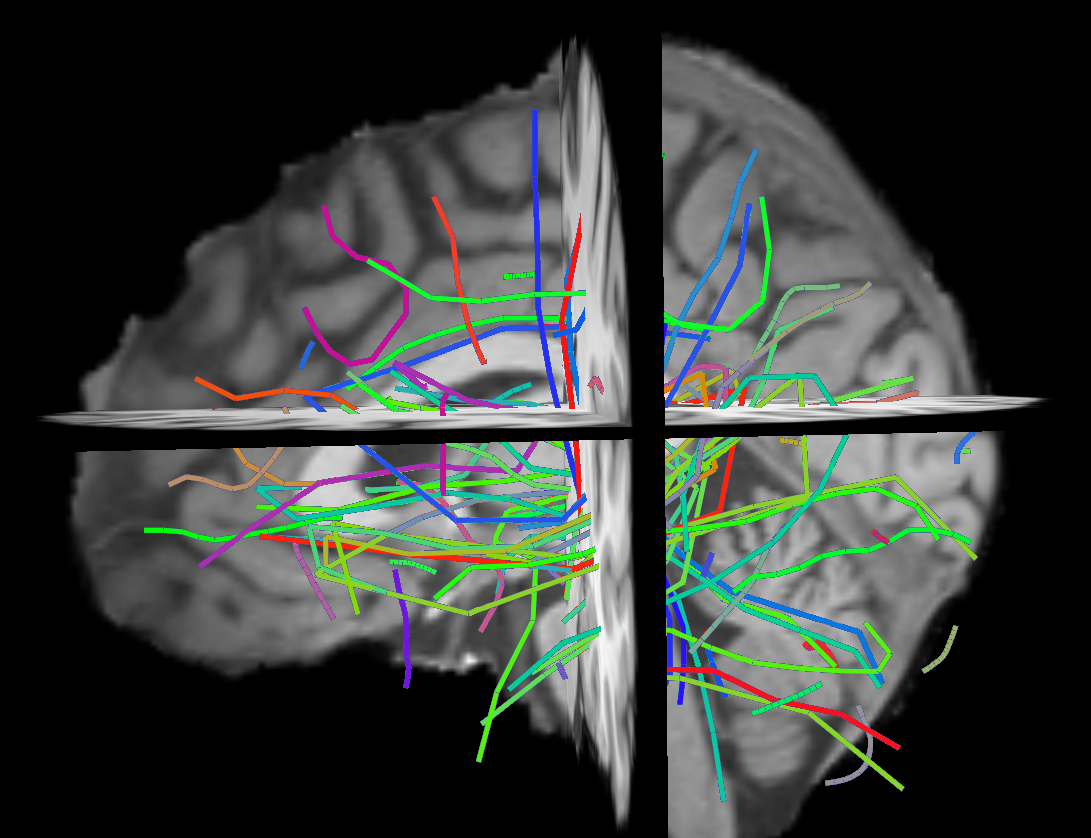
\includegraphics[width=3.2cm]{prni2012b.png}
  \caption{A set of $100$ streamlines, i.e. an example of prototypes, from a full tractography}
  \label{fig:streamlines}
\end{figure}
%copy and paste from the PRNI2012 - need to rewrite

The dissimilarity representation is an Euclidean embedding technique defined by selecting a set of objects (e.g. a set of streamlines) called prototypes, and then mapping any new object (e.g. any new streamline) to the vector of distances from the prototypes. Let have an $N$-streamline set $\mathcal{T} = \{s_1,\ldots,s_N\}$. 
%Let $P_{\mathcal{T}}$ be a probability distribution over $\mathcal{T}$. 
Let $d:\mathcal{T} \times
\mathcal{T} \mapsto \mathbb{R}^+$ be a distance function between two streamlines in $\mathcal{T}$. Note that $d$ is not assumed to be necessarily metric. Let $\Pi = \{\tilde{s}_1, \ldots, \tilde{s}_p\}$, where $\forall i$ $\tilde{s}_i \in \mathcal{\mathcal{T}}$ and $p$ is finite. We call each $\tilde{s}_i$ as \emph{prototype} or \emph{landmark}. The \emph{dissimilarity representation}/\emph{projection} is defined as $\phi_{\Pi}^d(s):\mathcal{\mathcal{T}} \mapsto \mathbb{R}^p$
s.t. 
\begin{equation}
  \phi_{\Pi}^d(s) = [d(s,\tilde{s}_1) ,\ldots, d(s,\tilde{s}_p)]
\label{eq:dissimilarity_representation}
\end{equation}
and maps a streamline $s$ from original space $\mathcal{T}$ to a vector of $\mathbb{R}^p$. 
%Note that this representation is a \emph{lossy} one in the sense that in general it is not possible to exactly reconstruct $X$ from $\phi_{\Pi}^d(X)$ because some information is lost during the projection. 
We define the distance between projected objects as the Euclidean distance between them: $\Delta_{\Pi}^d(s, s') = || \phi_{\Pi}^d(s) - \phi_{\Pi}^d(s') ||_2$, i.e. $\Delta_{\Pi}^d:\mathcal{T} \times \mathcal{T} \mapsto \mathbb{R}^+$. 
%It is intuitive 
Obviously, $\Delta_{\Pi}^d$ and $d$ should be strongly related.
Two main issues of the dissimilarity approximation lie on the strategies to choose prototypes (the number of prototypes and how to choose prototypes) and the measure of approximation to estimate the level of reconstruction $\mathcal{T}$ from $\phi_{\Pi}^d(\mathcal{T})$ (usually called \emph{lossy}). 

The issue of choosing the prototypes in order to achieve the desired degree of approximation usually bases on three popular selection policies: random selection, farthest first traversal (FFT) and subset farthest first (SFF)~\cite{turnbull2005fast}. 
\textit{Random policy} draws uniformly at random from $\mathcal{T}$, i.e. $\Pi \subseteq \mathcal{T}$ and $|\Pi|=p$.
\textit{FFT} selects an initial prototype at random from $\mathcal{T}$ and then each new one is defined as the farthest element of $\mathcal{T}$ from all previously chosen prototypes. 
FFT policy is related to the \emph{$k$-center} problem
%~\cite{hochbaum1985best}
: given a set $S$ and an integer $k$, what is the smallest $\epsilon$ for which you can find an $\epsilon$-cover\footnote{Given a metric space $(\mathcal{X},d)$, for any $\epsilon > 0$, an $\epsilon$-cover of a set $S \subset \mathcal{X}$ is defined to be any set $T \subset S$ such that $d(x,T) \leq \epsilon, \forall x \in S$. Here $d(x,T)$ is the distance from point $x$ to the closest point in set $T$} of $S$ of size $k$? \textit{SFF} policy samples $m = \lceil c p \log p \rceil$ points from $\mathcal{T}$ uniformly at random and then applies FFT on this sample in order to select the $p$ prototypes (c is an constant). All these policies are parametric with respect to the number of prototypes $p$. In the case of tractography, based on our experiments, SFF obtains an efficient and effective selection of the prototypes compared with two other methods~\cite{olivetti2012approximation}.
%As a measure of the degree of approximation of the dissimilarity representation, in the literature of the Euclidean embeddings of metric spaces, the term of \emph{distortion} is usually used~\cite{linial1995geometry}. It represents the relation between the distances in the original space and the corresponding ones in the projected space. 
%The embedding is said to have \emph{distortion}$\leq c$ if for every $x,x' \in \mathcal{X}$:
%\begin{equation}
%  \label{eq:distortion}
%  d(x,x') \geq \Delta_{\Pi}^d(x,x') \geq \frac{1}{c} d(x,x').
%\end{equation}
%Unfortunately this embedding is computationally too expensive to be used in practice. We investigate the relationship between the distribution of distances among objects in $\mathcal{X}$ through $d$ and the corresponding distances in the dissimilarity representation space through $\Delta_{\Pi}^d$. We claim that a good dissimilarity representation must be able to accurately preserve the partial order of the distances, i.e. if $d(X,X') \leq d(X,X'')$ then $\Delta_{\Pi}^d(X,X') \leq \Delta_{\Pi}^d(X,X'')$ for each $X,X',X'' \in \mathcal{X}$ almost always. 
\\As a measure of the degree of approximation of the dissimilarity representation, in the literature of the Euclidean embeddings of metric spaces, the term of \emph{distortion} is usually used~\cite{linial1995geometry}.
It represents the relation between the distances in the original space and 
%the corresponding ones 
in the projected space. 
The embedding is said to have \emph{distortion}$\leq c$ if for every $s,s' \in \mathcal{T}$:
\begin{equation}
  \label{eq:distortion}
  d(s,s') \geq \Delta_{\Pi}^d(s,s') \geq \frac{1}{c} d(s,s').
\end{equation}
However, this embedding is computationally too expensive to be used in practice. We investigate the relationship between the distribution of distances among streamlines in $\mathcal{T}$ through $d$ and the corresponding distances in the dissimilarity representation space through $\Delta_{\Pi}^d$. A good dissimilarity representation must be able to accurately preserve the partial order of the distances, i.e. if $d(s,s') \leq d(s,s'')$ then $\Delta_{\Pi}^d(s,s') \leq \Delta_{\Pi}^d(s,s'')$ for each $s,s',s'' \in \mathcal{T}$. We define the Pearson correlation %coefficient
$\rho$ between the two distances over all possible pairs of streamlines in $\mathcal{T}$:
\begin{equation}
  \label{eq:accuracy_correlation}
  \boldsymbol{\rho} = \frac{\mathrm{Cov}(d(s,s'),
    \Delta_{\Pi}^d(s,s'))}{\sigma_{d(s,s')} \sigma_{\Delta_{\Pi}^d(s,s')}}
\end{equation}
%where $s,s' \sim P_{\}$.  
An accurate correlation coefficient between
objects in $\mathcal{T}$ results in values of $\boldsymbol{\rho}$ far
from zero and close to $1$. The correlation focusses on the
\emph{averaged} differences between the original and projected space
while the distortion cares about the worst case scenario. For this reason, in our case, the correlation is a more appropriate measure. 
%In practical cases $P_X$ is unknown and only a finite sample $S$ is available. We can approximate $\boldsymbol{\rho}$ as the \emph{sample} correlation $\boldsymbol{r}$ where $X,X' \in S$. An accurate approximation of the relative distances between objects in $\mathcal{X}$ results in values of $\boldsymbol{\rho}$ far from zero and close to $1$\footnote{Note that negative correlation is not considered as accurate approximation. Moreover it never occurred during experiments}.

\subsection{Hierarchical clustering}%more on Eletherios thesis page 76
\label{subsec:hierarchical}
%\textbf{Reference more in \cite{schultz2011feature} pages 2 to 5} %thomas2011feature
%In the previous step, we use a set of example of the manual segmentaion to guide the segmentation procedure automatically through supervised learning. But the result of supervised segmentation is usually not satisfactory the requirement of doctors/neural scientists, and it is necessary to refine the segmentation. A clustering of some kind seems to be a solution to provide a useful technique to refine the segmentation. However, most of clustering algorithms return a flat unstructured set of clusters, require a prespecified number of clusters as input and are nondeterministic.  Moreover, most proposed clustering algorithms are very slow and often need to calculate pairwise distances of size $NxN$ where $N$ is the number of tracks. This amount of comparisons puts a massive load on clustering algorithms forcing them to be inefficient and therefore impractical for high frequency using as it is difficult to compute all these distances or even store them in memory. 
Hierarchical clustering~\cite{johnson1967hierarchical} produces a structure of clusters that is more informative than the unstructured set of clusters returned by flat clustering. This characteristic meets the requirement of creating an $m$-partition set $\mathbb{P}$ of $\mathcal{T}$ 
%the immediately responding to the changing level of abstraction of user 
without re-running the clustering algorithm again. Another advantage is that hierarchical clustering does not require to pre-specify the number of clusters. It builds nested clusters by merging them successively, and this hierarchy of clusters represented as a tree (or dendrogram). The root of the tree is the unique cluster that gathers all the samples, the leaves being the clusters with only one sample. In another way, hierarchical clustering algorithm
% (http://scikit-learn.org/stable/modules/clustering.html) 
can clusters data firstly on $N$ centers and consequently until only one center. This main character leads to the capability of visualizing $\mathcal{T}$ in many levels of abstraction, and the users can browse the value of level from $1$ to $N$, to see the clusters immediately.

With an $N$-streamline set $\mathcal{T} = \{s_1,\ldots,s_N\}$, hierarchical produces $Q$ clusters of $\mathcal{T}$
$H = \{H_{1}, \ldots, H_{Q}\}$, with $Q \leq N$, such that $C_{i} \in H_{m}, C_{j} \in H_{l}, m > l$
imply $C_{i} \in C_{j}$ or $C_{i} \cap C_{j} = \varnothing$, for all $i,j \neq i, m, l = 1, \ldots, Q$.
Hierarchical clustering algorithms are either top-down or bottom-up. Bottom-up algorithms treat each streamline as a singleton cluster at the outset and then successively merge (or agglomerate) pairs of clusters until all clusters have been merged into a single cluster that contains all tracts. Bottom-up hierarchical clustering is therefore called Hierarchical Agglomerative Clustering (HAC). Top-down clustering requires a method for splitting a cluster. It proceeds by splitting clusters recursively until individual streamlines are reached \cite{johnson1967hierarchical}.

Given an $N$-streamline set $\mathcal{T}$
%a set $\mathcal{T}$ of $N$ streamlines to be clustered, 
and an $N\times N$ (dis)similarity matrix, the basic process of HAC clustering~\cite{johnson1967hierarchical} is this:
\begin{enumerate}
	\item Assign each streamline to one cluster. We now have $N$ clusters, each containing just one streamline.
	%Let the distances (similarities) between the clusters the same as the distances (similarities) between the items they contain.
	\item Find the closest (most similar) pair of clusters and merge them into a single cluster.
	\item Compute distances (similarities) between the new cluster and each of the old clusters.
	\item Repeat steps $2$ and $3$ until all streamlines are clustered into a single cluster of size $N$.
\end{enumerate}
%$\mbox{   }\mbox{ }1.$ Assign each streamline to one cluster, and have $N$ clusters\\%, each containing just one streamline.\\
%$\mbox{   }\mbox{ }2.$ Find the closest (most similar) pair of clusters and merge\\
%$\mbox{          }$$\mbox{  }$$\mbox{  }$ them into a single cluster.\\
%$\mbox{   }\mbox{ }3.$ Compute distances (similarities) between the new cluster\\ 
%$\mbox{          }\mbox{ }\mbox{ }$ and each of the old clusters.\\
%$\mbox{   }\mbox{ }4.$ Repeat steps $2$ and $3$ until all streamlines are clustered\\
%$\mbox{          }\mbox{ }\mbox{ }$  into a single cluster of size $N$.
%Find the closest (most similar) pair of clusters and merge them into a single cluster, so that now you have one cluster less.
%Compute distances (similarities) between the new cluster and each of the old clusters.
%Repeat steps 2 and 3 until all items are clustered into a single cluster of size N. (*)
Step $3$ can be done in different ways, which distinguishes single-linkage, complete-linkage and average-linkage.
In \emph{single-linkage} clustering (also called the connectedness or minimum method), the distance between a pair of clusters $A$ and $B$ is the shortest distance from any streamline of one cluster to any streamline of the other cluster. 
%If the data consist of similarities, we consider the similarity between one cluster and another cluster to be equal to the greatest similarity from any member of one cluster to any member of the other cluster.
%${d}_sg(A,B) = \min_{i=1,\ldots,n_{s_A}} d({x}_i^A, s_B)$
\begin{equation}
\label{eq:distance_single_linkage}
d(A, B) = \min_{s_A \in {A},s_B \in {B}} d(s_A,s_B)
\end{equation}
where $d(s_A,s_B)$ is the distance between two streamlines:
\begin{equation}
\label{eq:distance_point_streamline}
d(s_A, s_B) = \min_{x_i^A \in s_A, x_j^B \in s_B}||{x}_i^A -{x}_j^B||_2
\end{equation}
with $x_i^A$ and $x_j^B$ are points belonging to streamline $s_A$ and $s_B$ respectively. 
In \emph{complete-linkage} clustering (also called the diameter or maximum method), we consider the distance between cluster $A$ and cluster $B$ to be equal to the greatest distance from any member of one cluster to any member of the other cluster.
\begin{equation}
\label{eq:distance_complete_linkage}
d(A, B) = \max_{s_A \in {A},s_B \in {B}} d(s_A,s_B)
\end{equation}
In \emph{average-linkage} clustering, the distance between two clusters $A$ and $B$ is defined as the average distance from any streamline of cluster $A$ to any streamline of cluster $B$.
\begin{equation}
\label{eq:distance_average_linkage}
d(A, B) = avg_{s_A \in {A},s_B \in {B}} d(s_A,s_B)
\end{equation}
In this project, we use the bottom-up hierarchical clustering (HAC strategy) combining with many distance measurements. The reason it that it is readily available to the fact that at the lowest level of abstraction, all streamlines should be presented, and when user changes the level of abstraction, some of present streamlines would be grouped and replaced by a representative. We hope that the HAC clustering can generate meaningful clusters with minimum memory consumption and respond in seconds with changes from user. However, HAC has not the capability to solve the problem of \emph{neighbor checking}. The solution for this problem is still under the investigation.
